\section{Auswertung}
\label{sec:Auswertung}
Die Formel für den Mittelwert lautet
 \begin{equation}
    \bar{x}=\frac{1}{n}\sum_{i=1}^n x_i.\\
\end{equation}
Die Standardabweichung wird mit folgender Formel
\begin{equation}
    s_x=\sqrt{\frac{1}{n-1}\sum_{i=1}^n {(x_i-\bar{x})^2 }}\\
\end{equation}
berechnet.
Die Formel für den Fehler des Mittelwertes lautet
\begin{equation}
    \Delta \bar{x} = s_{\bar{x}}=\frac{s_x}{\sqrt{n}}= \sqrt{\frac{1}{n(n-1)}\sum_{i=1}^n {(x_i-\bar{x})^2 }}.\\
\end{equation}
Diese werden im Folgenden verwendet.
\subsection{Programm und Geräteeinstellungen}
Um die Schallgeschwindigkeit zu bestimmen werden 2 Zylinder mit unterschiedlichen Grö"se verwendet. 
Die Länge der Zylinder werden mit der Schieblehre ausgemessen und betragen
\begin{align*}
    \text{für kleiner Zylinder}&: l_{\text{klein}} =39,5\, \text{mm}\\
    \text{für gro"ser Zylinder}&: l_{\text{gro"s}} =61,6\, \text{mm}.\\
   \end{align*}
Das Puls-Echo-Verfahren wird mit einem 39,5 mm-Acrylzylinder durchgefürht.
 Diese Messwerte und berechneten Werte sind in Tabelle \ref{tab:Programm} aufgelistet.

 \begin{table}[H]
    \centering
    \caption{Die Mess- und berechneten Daten zur Programm und Geräteeinstellungen.}
    \label{tab:Programm}
    \begin{tabular}{| c | c |c|c|  c |c|c|}
    \hline
    $\text{Länge/ mm} $ &\multicolumn{2}{c|}{$\text{Puls}\, 1$} & \multicolumn{2}{c|}{$\text{Puls}\, 2$}& $\Delta t/ \mu \text{s}$ &$c/ \text{(m/s)}$\\
    $\text{(Schieblehre)}$& $U/\text{V}$ & $t/ \mu \text{s}$ & $U/\text{V}$ & $t/ \mu \text{s}$ &{}&{}\\
    \hline
    39,5& 1,585& 0,6&0,09&29,6&29,0&2724,138\\
    \hline
\end{tabular}
\end{table}
\noindent
Die Länge des verwendeten Acrylzylinder ist durch Tiefenmessung bestimmt und beträgt 39,5 mm.
 Diese stimmt genau mit den mit der Schieblehre gemessenen Länge des Zylinders überein.
 Die berechnete Geschwindigkeit $c=2724,138 \,\text{m/s} $ in Acryl  wird in das Messprogramm eingetragen und die Messungen werden damit weiter durchgeführt.
\subsection{Bestimmung der Dämpfung mit dem Impuls-Echo-Verfahren}
In diesem Versuchteil wird die Dämpfung mit dem Impuls-Echo-Verfahren untersucht. Die Gleichung (4) beschreibt der Zusammenhang zwischen der Schallintensität I und der
durchlaufenen Wegstrecke $x$.
Mit $I \propto U^2$ gilt 
\begin{equation}
  U= U_0\, e^{\frac{-1}{2}\alpha x}.\\
   \end{equation}
Die Amplituden des ausgesendeten und des reflektierten Pulses (Spannungimpuls) werden gemessen und in Tabelle \ref{tab:Dmpfung} aufgelistet.
\begin{table}[H]
    \centering
    \caption{Die Messdaten zur Bestimmung der Dämpfung mit dem Impuls-Echo-Verfahren.}
    \label{tab:Dmpfung}
    \begin{tabular}{| c | c |c|}
    \hline
    $\text{Länge/ mm} $ &$\text{Puls}\, 1$ & $\text{Puls}\, 2$\\
   $\text{(Schieblehre)}$& $U/\text{V}$ & $U/\text{V}$ \\
    \hline
    39,5& 1,585&0,09\\
    61,6&1,602&0,045\\
    \hline
\end{tabular}
\end{table}
\noindent
 In Abbildung \ref{fig:Dämpfung} werden die Messdaten und Exponential-Regressionen grafisch dargestellt.
 \begin{figure}[H]
    \centering
    \includegraphics{Dämpfung.pdf}
    \caption{Die Regressionen zur Bestimmung der Dämpfung mit dem Impuls-Echo-Verfahren.}
    \label{fig:Dämpfung}
  \end{figure}
  \noindent
Die aus der Regression bestimmten
Werte fur die Absorptionskoeffizienten der Schallamplitude  bei 4MHz-Ultraschall lauten 
\begin{align*}
    \text{für kleiner Zylinder}:\,\, \alpha_{\text{klein}} &=\, 14,524\,\text{m}^{-1}\\
    \text{für gro"ser Zylinder}:\,\, \alpha_{\text{gro"s}} &=\, 11,599 \,\text{m}^{-1}\\
     \alpha &=(13,062\pm2,068)\, \text{m}^{-1}.\\
 \end{align*}

\subsection{Schallgeschwindigkeitsbestimmung mit dem Impuls-Echo-Verfahren}
Die Messdaten zur Schallgeschwindigkeitsbestimmung mit dem Impuls-Echo-Verfahren werden in Tabelle \ref{tab:Impuls} aufgelistet.
\begin{table}[H]
    \centering
    \caption{Die Mess und berechnete-Daten zur Schallgeschwindigkeitsbestimmung mit dem Impuls-Echo-Verfahren.}
    \label{tab:Impuls}
    \begin{tabular}{| c | c |c |c |}
    \hline
    $\text{Länge/ mm} $ &$\Delta t/ \mu \text{s}$&$\frac{\Delta t}{2}/ \mu \text{s}$ &$c/ \text{(m/s)}$\\
   $\text{(Schieblehre)}$& {}& {}& {}\\
    \hline
    39,5&29&14,5&2724,138 \\
    61,6&59&29,5&2088,136\\
    \hline
\end{tabular}
\end{table}
\noindent
Die Schallgeschwindigkeitsbestimmung mit dem Impuls-Echo-Verfahren beträgt dann $c= (2406,137\pm 449,721)\,\text{m/s}$.


\subsection{Schallgeschwindigkeitsbestimmung mit dem Durchschallungs-Verfahren}
 Die Messdaten \cite{1}  und berechneten Daten zur Schallgeschwindigkeitsbestimmung mit dem Durchschallungs-Verfahren werden in Tabelle \ref{tab:Durch} aufgelistet.
 \begin{table}[H]
    \centering
    \caption{Die Mess- und berechneten Daten zur Schallgeschwindigkeitsbestimmung mit dem Durchschallungs-Verfahren.}
    \label{tab:Durch}
    \begin{tabular}{| c | c |c |}
    \hline
    $\text{Länge/ mm} $ &$\Delta t/ \mu \text{s}$ &$c/ \text{(m/s)}$\\
   $\text{(Schieblehre)}$& {}& {}\\
    \hline
    39&22,5&1733,333 \\
    60&69,6&1515,152\\
    \hline
\end{tabular}
\end{table}
\noindent
Die Schallgeschwindigkeitsbestimmung mit dem Durchschallungs-Verfahren beträgt dann $c= (1624,243\pm 154,277)\,\text{m/s}$.


\subsection{Spektrale Analyse und Cepstrum}
Die Dicke der Polyacrylplatten werden mit der Schieblehre ausgemessen und betragen
\begin{align*}
    \text{für dicke Platte}&:\,\, d_{\text{dick}} =12,8\, \text{mm}\\
    \text{für dünne Platte}&:\,\, d_{\text{dünn}} =9,9\, \text{mm}.\\
   \end{align*}
Die dünnere Platte wird auf die dickere Platte gestellt. Der 39,5 mm lange Acrylzylinder wird dann auf die beiden Platten gestellt.
Das System wird mit dem Impuls-Echo-Verfahren so untersucht, dass drei Mehrfachreflexionen zu sehen sind.
Mit Hilfe  der FFT- Funktion  werden das Spektum und Ceptrum der Sonde für die ersten drei Peaks erstellt. (siehe Abbildung \ref{fig:cepstrum})
Daraus ist es ersichtlich, dass sich dem Signal der Sonde
nun die Mehrfachreflexe überlagern. Die Peaks liegen ungerfähr bei den Stellen, an deren Länge/Dicke vom Zylinder bzw. zwei Platten entsprechen.
Aus der Abbildung und mit Hilfe der Tiefenmessung  werden die Dicken durch Gleichung (6) der Platten bestimmt.
(Hier wird die Schallgeschwindigkeit $c=2724,138\, \text{m/s} $ aus 4.1 verwendet.) 
Die Messdaten \cite{1}  und berechnete Daten werden in Tabelle \ref{tab:Ceptrum} aufgelistet.
\begin{table}[H]
   \centering
   \caption{Die Mess- und berechneten Daten zur Bestimmung der Dicken der Polyacrylplatten .}
   \label{tab:Ceptrum}
   \begin{tabular}{| c | c |c |}
   \hline
  $\Delta t/ \mu \text{s}$ &$\text{Dicke/ mm} $ \\
   \hline
   7,3&9,943\\
   \hline
   8,7&11,850\\
   \hline
\end{tabular}
\end{table}

\begin{figure}
    \centering
    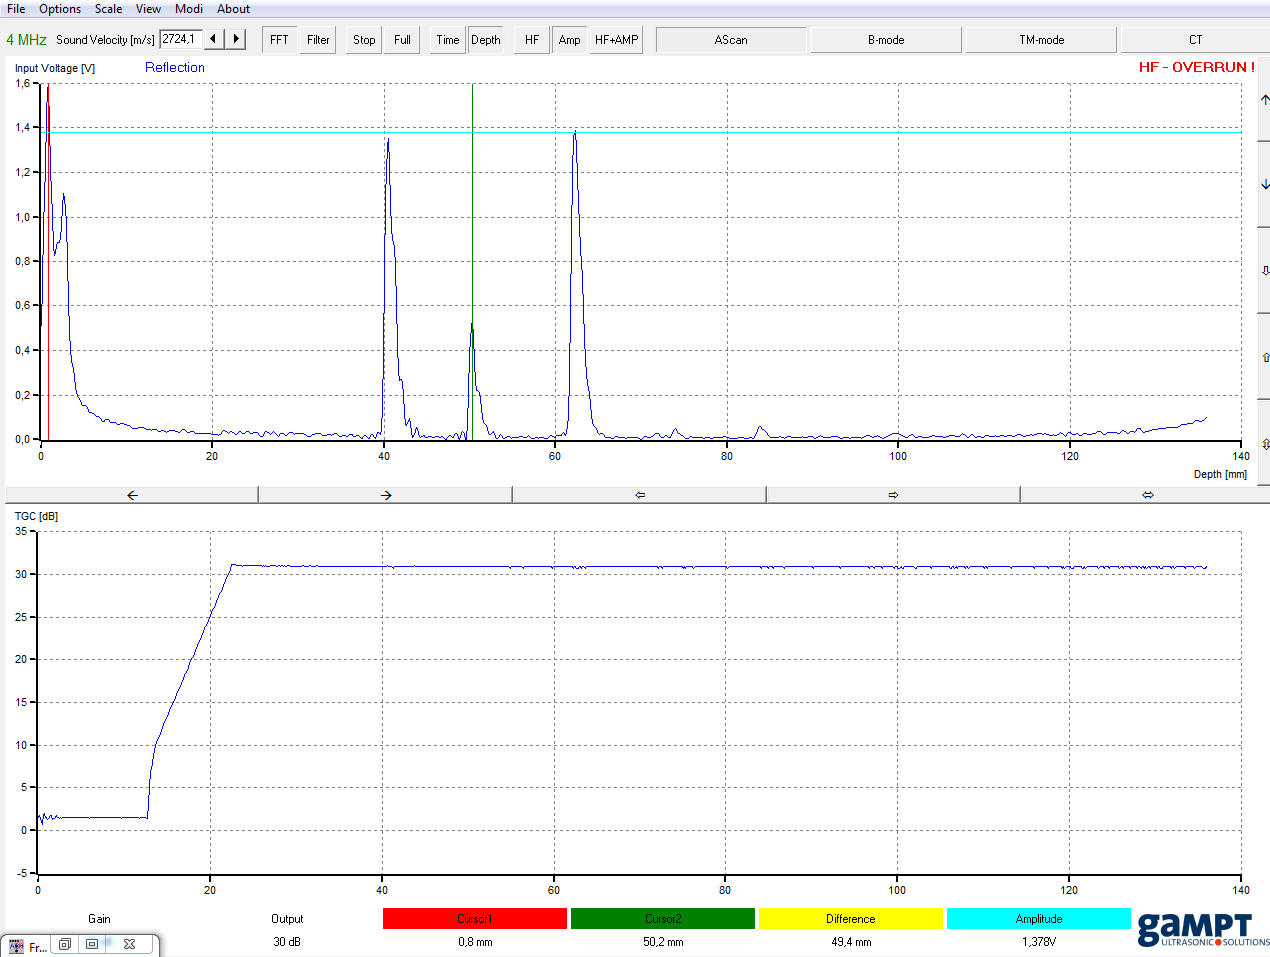
\includegraphics[width=\textheight,height=\textwidth,angle=90]{stapel1.png}
    \caption{Stapel.}
    \label{fig:stapel}
\end{figure}

\begin{figure}
    \centering
    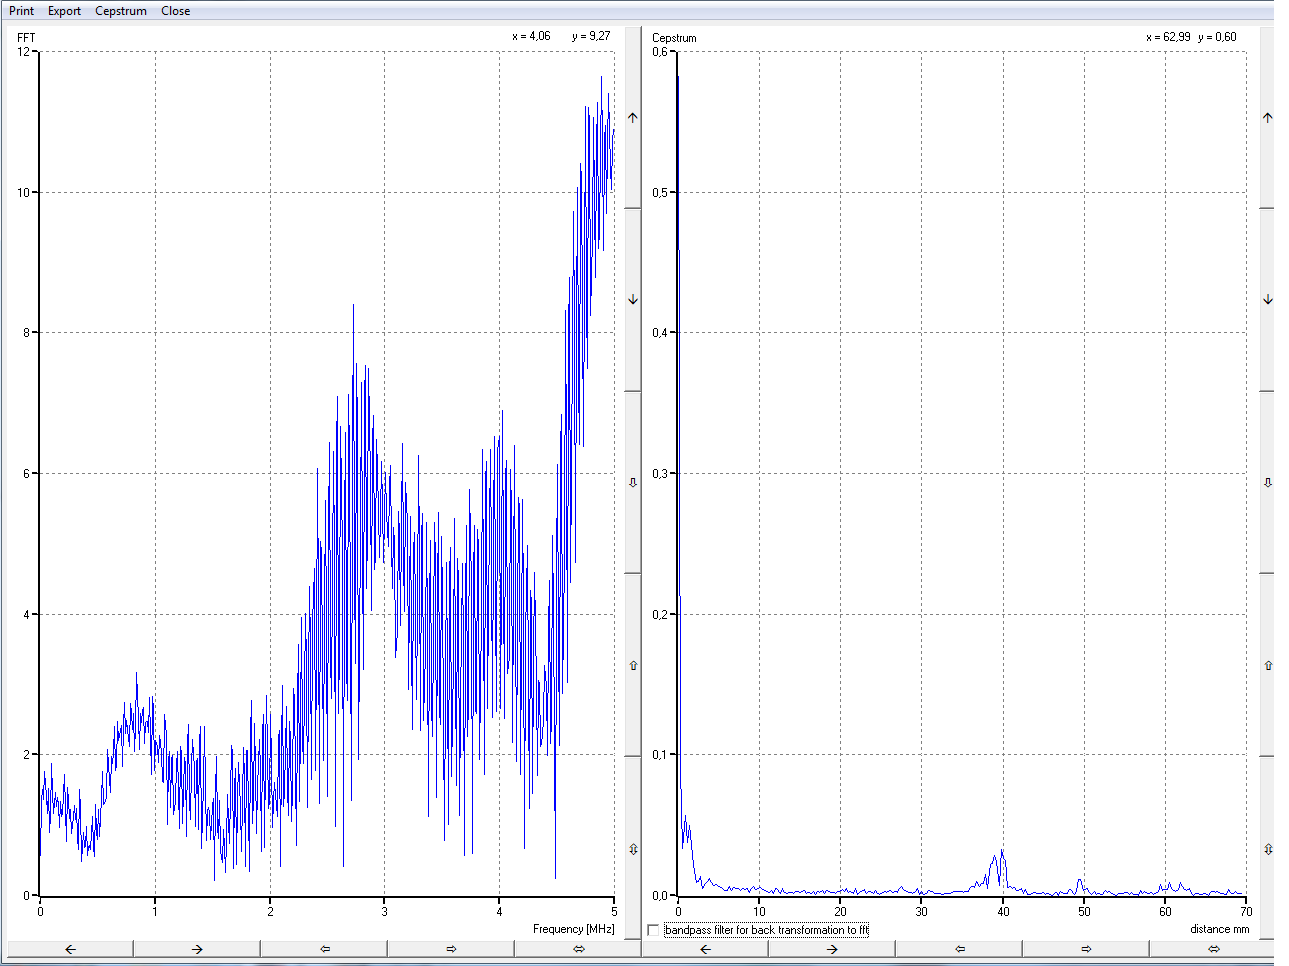
\includegraphics[width=\textheight,height=\textwidth,angle=90]{cepstrum1.png}
    \caption{Cepstrum.}
    \label{fig:cepstrum}
\end{figure}
 